\documentclass[../main.tex]{subfiles}

\graphicspath{{\subfix{../imgs/}}}

\begin{document}

\section{Embedded System X}

The objective of the assignment is to implement \texttt{Embedded System X} (Figure \ref{fig:esx_state_diagram}) using four different design patterns. \texttt{Embeddded System X} will be implemented using the following design patterns.

\begin{enumerate}
    \item Singleton pattern
    \item Command pattern
    \item State pattern
    \item Active object pattern
\end{enumerate}

\begin{figure}[h]
    \centering
    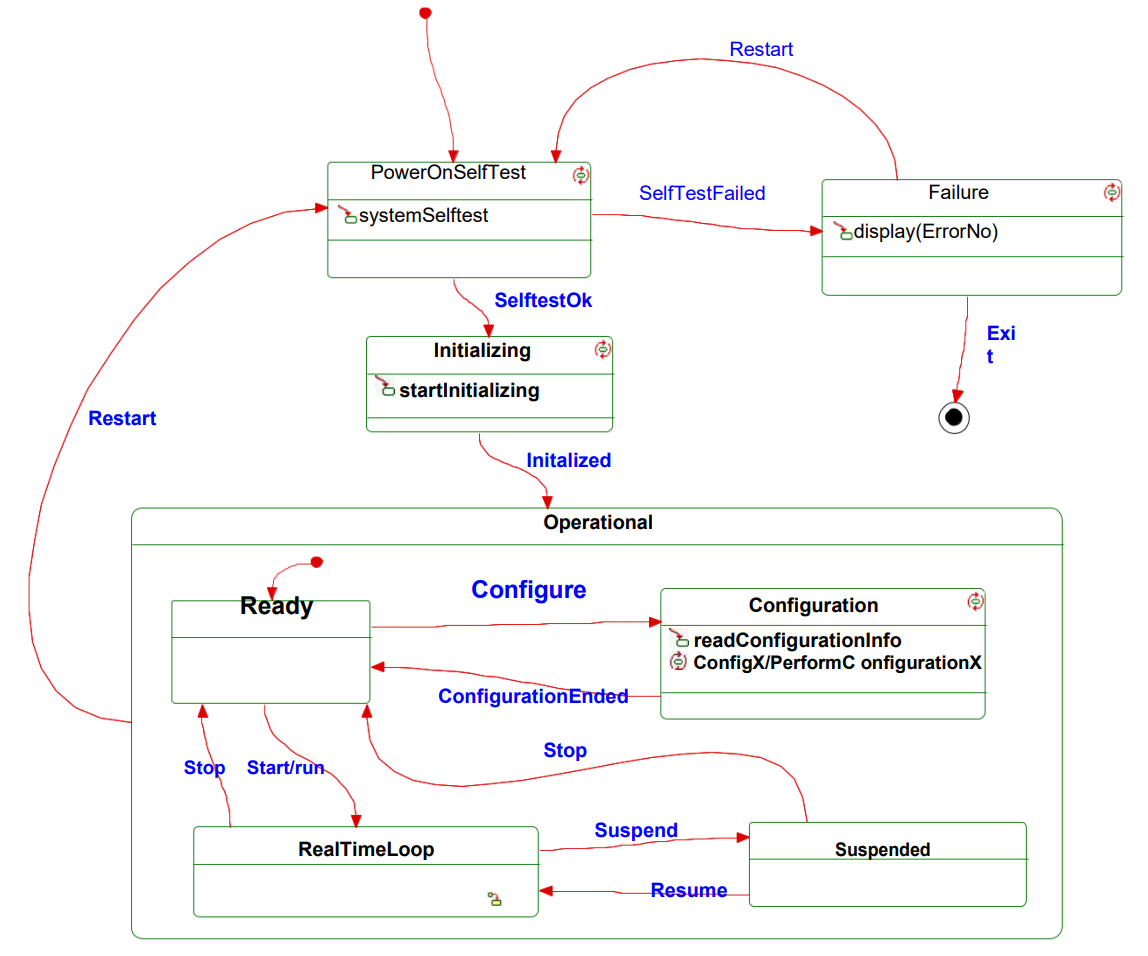
\includegraphics[width=0.8\textwidth]{esx_state_diagram.png}
    \caption{State diagram of Embedded System X.}
    \label{fig:esx_state_diagram}
\end{figure}

\subsection{Singleton Pattern}

For the state classes, we used the singleton pattern to assure only one instance of each class exists at all times in the system. This simplifies the implementation of the state pattern, as we can use the same instance of the state class in the context class. It also reduces the memory usage. 

\vspace{10pt}
Each state class has a public method \texttt{getInstance()} that returns the instance of the class. If the instance is not created, it will create a new instance and return it.

\begin{myminted}{Initialization state singleton pattern}
static Initializing* getInstance() {
    if(instance == nullptr) {
        instance = new Initializing();
    }
    return instance;
}
\end{myminted}

\newpage

\subsection{State Pattern}

This pattern is used to \textit{manage} the various states of the system. Each state is a subclass of the abstract class \texttt{State}. The context class \texttt{EmbeddedSystemX} has a reference to the current state. The context class has methods that handle the events that change the state of the system. This design pattern allows the system to change its behavior when its state changes.

\begin{myminted}{Abstract state class}
class State {
    public:
    virtual void selfTestOk(EmbeddedSystemX* context){};
    virtual void selfTestFailed(EmbeddedSystemX* context, int errorNo){};
    virtual void restart(EmbeddedSystemX* context){};
    virtual void exit(EmbeddedSystemX* context){};
    virtual void initialized(EmbeddedSystemX* context){};
    virtual void configure(EmbeddedSystemX* context){};
    virtual void configurationEnded(EmbeddedSystemX* context){};
    virtual void start(EmbeddedSystemX* context){};
    virtual void stop(EmbeddedSystemX* context){};
    virtual void suspend(EmbeddedSystemX* context){};
    virtual void resume(EmbeddedSystemX* context){};
    virtual string getStateName() const = 0;
    virtual ~State() = default;
};
\end{myminted}

\subsection{Command Pattern}

The events \texttt{Resume} and \texttt{Stop} in the \texttt{Suspended} state are implemented using the command pattern. Each occurence of these events creates a request object.

\begin{myminted}{Command pattern for resume}
void EmbeddedSystemX::resume() {
    CommandResume req(&(this->state));
    req.execute();
}
\end{myminted}

\subsection{Active Object Pattern}

The \texttt{RealTimeLoop} is treated as an active object. This pattern allows for the creation of request objects for each event (e.g., chMode1, chMode2, chMode3). Each request object calls the corresponding handler method from the source state, enabling asynchronous processing of events.

\newpage

\section{Real Time Loop}

The Real Time Loop is implemented using the state pattern, active object pattern, and command pattern. The state diagram of the Real Time Loop is shown in Figure \ref{fig:rtl_state_diagram}. The class diagram is shown in Figure \ref{fig:rtl_implementation}.

\begin{figure}[h]
    \centering
    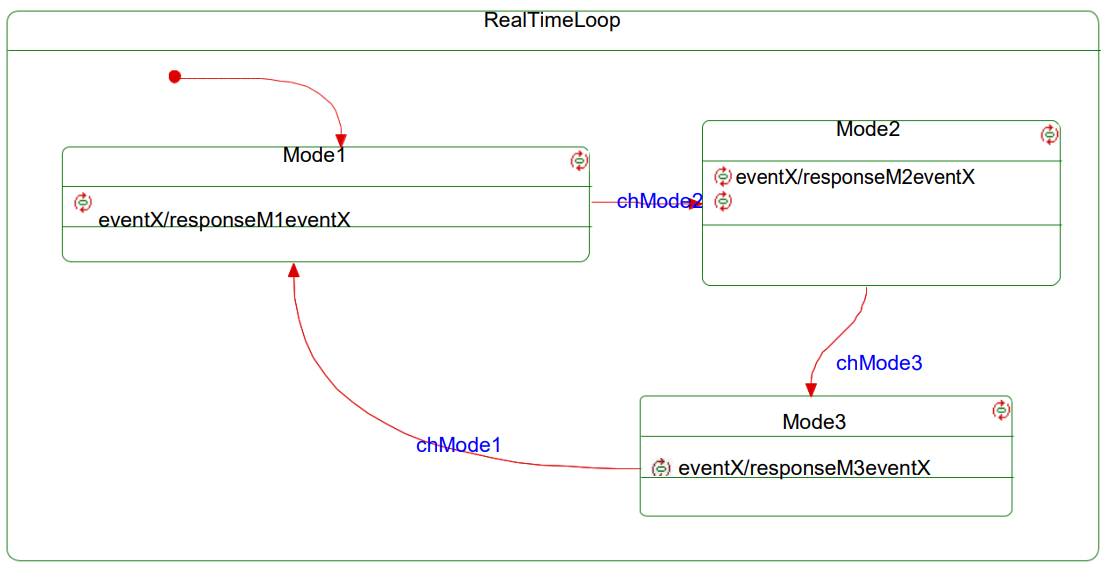
\includegraphics[width=0.9\textwidth]{realtimeloop.png}
    \caption{State diagram of Real Time Loop.}
    \label{fig:rtl_state_diagram}
\end{figure}

\begin{figure}[h]
    \centering
    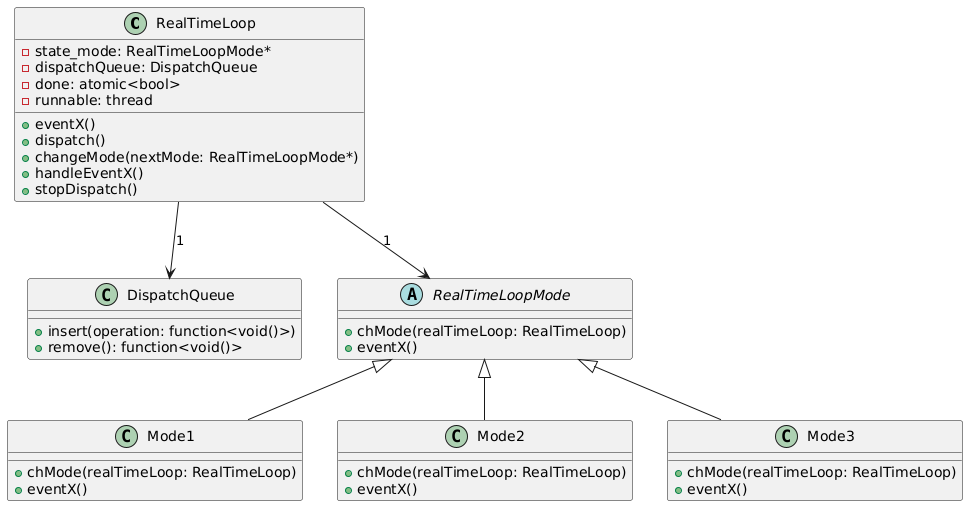
\includegraphics[width=0.9\textwidth]{realtimeloop_uml.png}
    \caption{Class diagram of Real Time Loop.}
    \label{fig:rtl_implementation}
\end{figure}

\newpage

\section{Implementation}

\begin{mintedterminal}
Test program...
Current state   Next state
PowerOnSelfTest Initializing

Current state   Next state
Initializing    Ready

Current state   Next state
Ready           Configuration

Current state   Next state
Configuration   Ready

Current state   Next state
Ready           RealTimeLoop

Current state   Next state
RealTimeLoop    Suspended

Resuming to RealTimeLoop state.
Stopping and transitioning to Ready state.
Testing RealTimeLoop Active Object...
Triggering eventX in Mode1...
DispatchQueue: Inserted operation.
Dispatch loop started.
DispatchQueue: Removed operation.
RealTimeLoop: Handling eventX in 5Mode1
Mode1 eventX

Switching to Mode2...
RealTimeLoop: Changed mode to 5Mode2
Triggering eventX in Mode2...
DispatchQueue: Inserted operation.
DispatchQueue: Removed operation.
RealTimeLoop: Handling eventX in 5Mode2
Mode2 eventX

Switching to Mode3...
RealTimeLoop: Changed mode to 5Mode3
Triggering eventX in Mode3...
DispatchQueue: Inserted operation.
DispatchQueue: Removed operation.
RealTimeLoop: Handling eventX in 5Mode3
Mode3 eventX

Stopping RealTimeLoop dispatch thread...
DispatchQueue: Inserted operation.
DispatchQueue: Removed operation.
Dispatch loop exited.
Dispatch thread stopped.
All tests completed.
\end{mintedterminal}

\end{document}